\documentclass[a4paper,12pt]{report}

% Packages
\usepackage{graphicx}
\usepackage{algorithm}
\usepackage{algpseudocode}
\usepackage{booktabs}
\usepackage{listings}
\usepackage{xcolor}
\usepackage{amsmath,amssymb,amsfonts}
\usepackage{hyperref}
\usepackage{geometry}
\geometry{a4paper, top=2.5cm, bottom=2.5cm, left=2.5cm, right=2.5cm}

% Persian support
\usepackage{xepersian}
\settextfont{XB Zar} % Standard academic Persian font (use Yas or IRANSans if preferred)
\setlatintextfont{Times New Roman}
\setdigitfont{XB Zar}

% Listings style for code snippets
\lstset{
  basicstyle=\footnotesize\ttfamily,
  breaklines=true,
  frame=single,
  backgroundcolor=\color{gray!5},
  keywordstyle=\color{blue}\bfseries,
  commentstyle=\color{green!50!black},
  numberstyle=\tiny,
  numbers=left,
  numbersep=6pt,
  direction=RTL
}

% --------------------------------------------------
% Title Page
% --------------------------------------------------
\begin{document}

\begin{titlepage}
\begin{center}
\vspace*{1cm}

{\Large \textbf{دانشگاه شهید بهشتی}}\\
\vspace{0.5cm}
{\large \textbf{دانشکده مهندسی و علوم کامپیوتر}}\\
\vspace{2cm}

{\Large \textbf{عنوان پروژه:}}\\
\vspace{0.5cm}
{\LARGE \textbf{نگهبان خطا: مدل‌های زبانی کوچک کارآمد برای تولید توضیحات شطرنج با هدایت اکتشافی}}\\
\vspace{1cm}
{\large (Blunder Guard: Efficient Small Language Models for Heuristic-Guided Chess Commentary Generation)}\\
\vspace{2cm}

{\large \textbf{پروژه کارشناسی}}\\
\vspace{2cm}

{\large \textbf{دانشجو:}}\\
{\large سید علی حسین‌نساب}\\
\vspace{1cm}

{\large \textbf{استاد راهنما:}}\\
{\large دکتر مریم طهماسبی}\\
\vspace{2cm}

{\large \textbf{فصل و سال دفاع:}}\\
{\large تابستان ۱۴۰۳}\\ % Adjust the semester/year as needed

\vfill
\end{center}
\end{titlepage}

% --------------------------------------------------
% Abstract
% --------------------------------------------------
\chapter*{چکیده}
\addcontentsline{toc}{chapter}{چکیده}
ما در این پروژه \textbf{نگهبان خطا} (Blunder Guard) را معرفی می‌کنیم، یک سیستم قابل استقرار محلی برای تولید توضیحات آموزشی شطرنج با ادغام یک مدل زبانی کوچک (SLM) سازگار شده با دامنه و ارزیابی کلاسیک موتور شطرنج. یک مدل Qwen3 با ۱.۷ میلیارد پارامتر بر روی متون کلاسیک و بدون ساختار شطرنج تنظیم دقیق شده و در زمان استنتاج توسط ویژگی‌های قطعی، ارزیابی‌ها و تغییرات اصلی مشتق شده از Stockfish هدایت می‌شود.

پیکره آموزشی شامل بیش از ۲.۸ میلیون توکن استخراج شده از کتاب‌های مرجع شطرنج با استفاده از یک خط لوله موازی استخراج PDF است. ویژگی‌های موقعیتی از ارزیابی‌های Stockfish محاسبه و از طریق یک استخراج‌کننده ویژگی ساختاریافته پردازش می‌شوند. مدل برای استقرار با \texttt{llama.cpp} به فرمت GGUF صادر می‌شود؛ نقطه وزن تنظیم‌شده ارزیابی‌شده در این گزارش از کمی‌سازی Q8\_0 استفاده می‌کند.

ما یازده مدل زبانی نامزد را بر روی ۶۰ انتقال موقعیت نگهداری‌شده که به طور مساوی بین سطوح مبتدی، متوسط و پیشرفته تقسیم شده‌اند، ارزیابی می‌کنیم. یک مدل ۱۲ میلیارد پارامتری از خانواده Gemma به عنوان داور محلی عمل کرده و صحت، پیروی از دستورالعمل، سودمندی، وفاداری و روانی را در مقابل مراجع معتبر امتیازدهی می‌کند. مدل تنظیم‌شده ما روان است اما در مجموع تنها ۲.۴۹ از ۱۰ امتیاز کسب می‌کند، در حالی که قوی‌ترین مدل میزبان آزمایش‌شده ۷.۳۱ از ۱۰ را کسب می‌کند. نتایج نشان می‌دهد که استقرار محلی عملی است، اما روانی متن به تنهایی صحت مبتنی بر شطرنج را تضمین نمی‌کند.

\vspace{0.5cm}
\noindent \textbf{واژگان کلیدی:} هوش مصنوعی شطرنج، مدل‌های زبانی کوچک، هوش مصنوعی توضیح‌پذیر، تولید زبان طبیعی، ارزیابی محلی.

% --------------------------------------------------
% Table of Contents
% --------------------------------------------------
\tableofcontents
\newpage

% --------------------------------------------------
% Chapter 1
% --------------------------------------------------
\chapter{کلیّات}
\section{مقدمه}
همگرایی موتورهای شطرنج فوق‌انسانی و تولید زبان طبیعی، فرصتی منحصر‌به‌فرد برای آموزش شطرنج فراهم می‌کند: توضیح \emph{چرایی} برتری یک موقعیت به زبانی که برای یادگیرندگان انسانی قابل درک باشد. موتورهای مدرن مانند Stockfish و AlphaZero به دقت تاکتیکی فراتر از استادان بزرگ دست می‌یابند، اما خروجی آن‌ها (ارزیابی‌های سانتی‌پیawn و تغییرات اصلی) برای بازیکنان متوسط مبهم باقی می‌ماند. از سوی دیگر، مدل‌های زبانی بزرگ (LLM) توضیحات روانی تولید می‌کنند اما اغلب دچار توهم تاکتیکی شده و موقعیت‌ها را اشتباه ارزیابی می‌کنند که آن‌ها را برای آموزش جدی غیرقابل اعتماد می‌سازد.

این کار به مسئله \textbf{تحلیل شطرنج تفسیرپذیر} می‌پردازد: تولید توضیحاتی که همزمان (۱) از نظر استراتژیک دقیق و مبتنی بر ارزیابی عینی موتور باشند؛ (۲) از نظر آموزشی ساختاریافته و پیرو قراردادهای متون کلاسیک شطرنج باشند؛ و (۳) از نظر محاسباتی کارآمد بوده و استقرار کاملاً محلی را بدون وابستگی به فضای ابری امکان‌پذیر سازند.

\section{بیان مسئله}
بسیاری از بازیکنان شطرنج (از باشگاه‌ها تا افراد) به دنبال ابزارهای مربی‌گری مقرون‌به‌صرفه و خصوصی هستند. روش‌های موجود به دو دسته تقسیم می‌شوند: روش‌های نظارت‌شده که به مجموعه داده‌های بزرگ حاشیه‌نویسی‌شده نیاز دارند و مقیاس‌پذیر نیستند، و روش‌های مبتنی بر LLM که از طریق مقیاس به کیفیت می‌رسند اما هزینه‌های بالایی داشته و نگرانی‌های حریم خصوصی را مطرح می‌کنند. هیچ‌یک از این رویکردها نیازهای بازیکنان برای یک ابزار تحلیل محلی، سبک و قابل اعتماد را برآورده نمی‌کنند. چالش اصلی این است که چگونه می‌توان دانش استراتژیک عمومی را از متون شطرنج آموخت و آن را با ارزیابی‌های دقیق و قطعی یک موتور شطرنج ترکیب کرد تا توضیحاتی تولید شود که هم آموزنده باشند و هم از نظر تاکتیکی صحیح.

\section{کلیات روش پیشنهادی}
ما پارادایم متفاوتی را پیشنهاد می‌کنیم: تنظیم دقیق مدل‌های زبانی کوچک (SLM) بر روی متون بدون ساختار شطرنج، در حالی که تولید متن با اکتشافات تأییدشده توسط موتور هدایت می‌شود. متون آموزشی کلاسیک الگوهای توضیحی قابل استفاده مجدد را بدون برچسب‌های خاص موقعیت کدگذاری می‌کنند. با یادگیری این الگوها، یک SLM می‌تواند هنگامی که توسط اولویت‌های اکتشافی مشتق شده از Stockfish هدایت می‌شود، به موقعیت‌های جدید تعمیم یابد.
مراحل کلی روش پیشنهادی عبارتند از:
\begin{enumerate}
    \item استخراج و پاک‌سازی متون از کتاب‌های مرجع شطرنج.
    \item تنظیم دقیق مدل پایه (Qwen3-1.7B) با استفاده از QLoRA برای بهینه‌سازی مصرف حافظه.
    \item کمی‌سازی مدل به فرمت Q8\_0 با استفاده از \texttt{llama.cpp} برای استقرار کارآمد روی سخت‌افزار مصرف‌کننده.
    \item استخراج ویژگی‌های ساختاری (مانند تغییرات ارزیابی، ایمنی شاه، ساختار پیاده) از دو موقعیت FEN (قبل و بعد از حرکت) توسط Stockfish.
    \item تولید توضیح نهایی توسط مدل با استفاده از یک پرامپت ساختاریافته که شواهد موتور را در بر دارد اما از به کار بردن اصطلاحات فنی موتور در خروجی نهایی جلوگیری می‌کند.
\end{enumerate}

\section{ساختار پروژه}
این گزارش در سه فصل سازماندهی شده است. فصل اول به کلیات، بیان مسئله و نمای کلی روش پیشنهادی پرداخت. فصل دوم مفاهیم پایه (مانند موتورهای شطرنج، مدل‌های زبانی کوچک و کمی‌سازی) و کارهای مرتبط پیشین را مرور می‌کند. فصل سوم به جزئیات روش پیشنهادی، آماده‌سازی داده‌ها، پروتکل ارزیابی، ارائه نتایج کمی بر اساس مدل داور و در نهایت بحث و نتیجه‌گیری می‌پردازد.

% --------------------------------------------------
% Chapter 2
% --------------------------------------------------
\chapter{مفاهیم پایه و کارهای مرتبط}
\section{مقدمه}
در این فصل، ابتدا تصویری جامع از مفاهیم پایه که مبنای این پروژه هستند ترسیم می‌شود. سپس، ارتباط میان این مفاهیم و نحوه تأثیرگذاری آن‌ها بر یکدیگر تبیین می‌گردد. در بخش دوم، کارهای مرتبط موجود (پژوهشی و تجاری) بررسی شده و نقاط قوت، ضعف و تمایز روش پیشنهادی این پروژه نسبت به آن‌ها مشخص می‌شود.

\section{مفاهیم پایه}
\subsection{موتورهای شطرنج و ارزیابی موقعیت}
موتورهایی مانند Stockfish با استفاده از الگوریتم Minimax و هرس Alpha-Beta به همراه توابع ارزیابی عصبی (NNUE)، موقعیت‌ها را تا عمق زیاد جستجو کرده و امتیازی بر حسب سانتی‌پیawn و لیستی از بهترین ادامه‌ها (Principal Variations) ارائه می‌دهند.

\subsection{مدل‌های زبانی کوچک (SLM) و QLoRA}
مدل‌های زبانی کوچک (زیر ۱۰ میلیارد پارامتر) تعادلی بین عملکرد و کارایی محاسباتی ایجاد می‌کنند. QLoRA (Quantized Low-Rank Adaptation) با کمی‌سازی وزن‌های پایه به ۴ بیت و افزودن آداپتورهای رتبه پایین قابل آموزش، تنظیم دقیق را روی سخت‌افزارهای مصرف‌کننده امکان‌پذیر می‌سازد.

\subsection{کمی‌سازی و \texttt{llama.cpp}}
کمی‌سازی فرآیند کاهش دقت اعداد (مثلاً از FP16 به INT8) برای کاهش حجم مدل و سرعت بخشیدن به استنتاج است. \texttt{llama.cpp} چارچوبی بهینه برای اجرای مدل‌های فرمت GGUF روی CPU و GPU فراهم می‌کند.

\section{کارهای مرتبط}
جدول \ref{tab:related-comparison} مقایسه‌ای با نزدیک‌ترین سیستم‌های توضیح و تولید نظر شطرنج را نشان می‌دهد.

\begin{table}[htbp]
\centering
\caption{مقایسه با نزدیک‌ترین سیستم‌های تولید توضیحات شطرنج}
\label{tab:related-comparison}
\begin{tabular}{@{}p{2.2cm}p{2.2cm}p{2.2cm}p{2.2cm}p{2.5cm}@{}}
\toprule
\textbf{پژوهش} & \textbf{پایه شطرنجی} & \textbf{نظارت زبانی} & \textbf{ارزیابی} & \textbf{تمایز اصلی با نگهبان خطا} \\
\midrule
Jhamtani et al. & ویژگی‌های دستی و امتیاز موتور & ۲۹۸ هزار جفت نظر & معیارهای خودکار و مطالعه انسانی & تولید نظارت‌شده آگاه از ویژگی \\
Zang et al. & موتور عصبی شطرنج مشترک & نظرات جفت‌شده بر اساس دسته & خودکار و انسانی & بازنمایی پیوسته داخلی موتور \\
Lee et al. & برچسب‌های کنترلی نمادین & وضعیت‌ها و نظرات جفت‌شده & Perplexity و ترجیح انسانی & معماری نزدیک؛ رابط کنترل گسسته آموخته‌شده \\
Kim et al. & مفاهیم اولویت‌بندی‌شده از مدل خبره & تولید توسط LLM بزرگ & انسانی و GCC-Eval & اولویت‌بندی مفهوم و داور LLM \\
نگهبان خطا & چند-PV استوک‌فیش و دلتای صفحه & کتاب‌های شطرنج جفت‌نشده؛ پرامپت محدود & مراجع امتیازدهی‌شده توسط Gemma-4-12B محلی & تولیدکننده کوچک محلی و رابط ویژگی بازرسی‌پذیر \\
\bottomrule
\end{tabular}
\end{table}

\section{جمع‌بندی}
مرور کارهای پیشین نشان می‌دهد که اگرچه روش‌های نظارت‌شده دقت بالایی دارند، اما به داده‌های برچسب‌دار گران‌قیمت نیاز دارند. روش پیشنهادی ما با استفاده از دانش عمومی استخراج‌شده از کتاب‌ها و هدایت اکتشافی در زمان استنتاج، شکاف بین دقت موتور و روانی زبان را بدون نیاز به داده‌های جفت‌شده پر می‌کند.

% --------------------------------------------------
% Chapter 3
% --------------------------------------------------
\chapter{روش پیشنهادی و نتایج ارزیابی}
\section{مقدمه}
در این فصل، جزئیات طراحی و پیاده‌سازی سیستم نگهبان خطا، شامل آماده‌سازی مجموعه داده، معماری روش پیشنهادی، پروتکل ارزیابی و در نهایت تحلیل نتایج کمی ارائه می‌شود.

\section{آماده‌سازی مجموعه داده}
\subsection{پیکره آموزشی}
مجموعه داده آموزشی شامل متون دیجیتال‌شده از پنج کتاب مرجع شطرنج (مانند آثار تاراش، برنشتاین، تال، سیلمن و چرنیو) است. یک خط لوله موازی با استفاده از \texttt{pypdf} برای استخراج متن، حذف خط‌شکن‌ها و عادی‌سازی فاصله‌ها توسعه یافت که منجر به استخراج حدود ۲.۸ میلیون توکن تمیز شد.

\subsection{ماژول بهبود اکتشافی}
برای هدایت تولید در زمان استنتاج، یک ماژول اکتشافی، دو موقعیت FEN (قبل و بعد از حرکت) را با استفاده از Stockfish (عمق ۱۷، ۳ تغییر اصلی) تحلیل می‌کند. این ماژول تغییرات ساختاری قطعی مانند ایمنی شاه، ساختار پیاده، کنترل مرکز و ایمنی مهره‌ها را استخراج کرده و در یک پرامپت ساختاریافته بسته‌بندی می‌کند.

\section{روش پیشنهادی}
\subsection{معماری سیستم}
شکل \ref{fig:structure} نمای کلی سیستم را نشان می‌دهد. API پیاده‌سازی‌شده دو رشته FEN را دریافت می‌کند، Stockfish هر دو موقعیت را تحلیل می‌کند، لایه شطرنج پایتون دلتاهای ساختاری را استخراج می‌کند و شواهد حاصل در یک پرامپت محدود و مناسب برای مبتدیان سریال‌سازی می‌شود.

\begin{figure}[htbp]
    \centering
    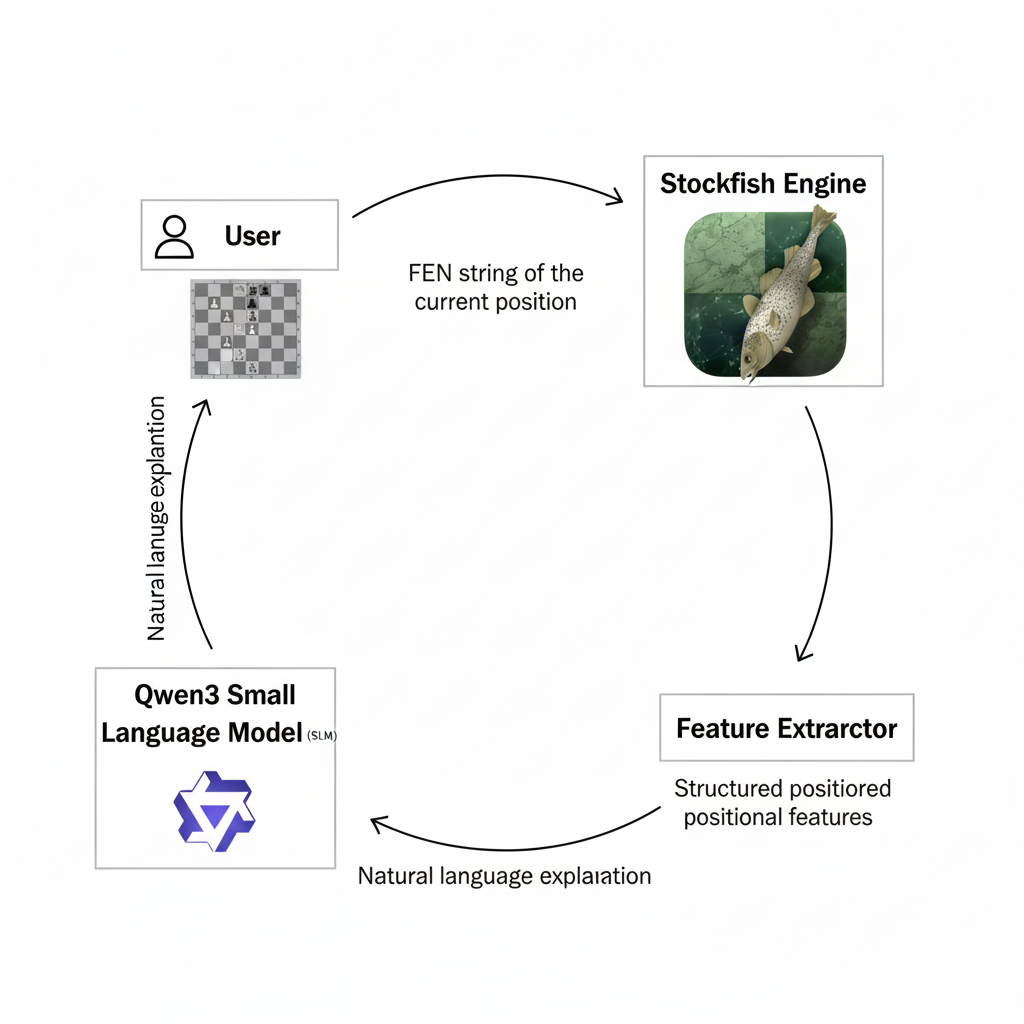
\includegraphics[width=0.8\textwidth]{structure_diagram.png}
    \caption{معماری سیستم. پیاده‌سازی فعلی یک انتقال موقعیت را به جای یک صفحه ایزوله تحلیل می‌کند.}
    \label{fig:structure}
\end{figure}

\subsection{تنظیم دقیق و کمی‌سازی}
مدل پایه \textbf{Qwen3-1.7B} با استفاده از QLoRA (رتبه $r=16$، $\alpha=32$) بر روی پیکره متنی تنظیم دقیق شد. پس از آموزش، آداپتورهای LoRA با مدل پایه ادغام و مدل حاصل با استفاده از \texttt{llama.cpp} به فرمت Q8\_0 کمی‌سازی شد تا برای استنتاج روی سخت‌افزار محدود بهینه شود.

\section{روش ارزیابی}
معیارهای استاندارد تولید زبان طبیعی (مانند BLEU یا ROUGE) برای این کار مناسب نیستند، زیرا پیکره آموزشی ما فاقد داده‌های جفت‌شده موقعیت-نظر است. در عوض، ما از پارادایم \textbf{LLM-as-a-judge} استفاده می‌کنیم.
ما ۶۰ انتقال موقعیت از پایگاه داده Lichess (۲۰ مبتدی، ۲۰ متوسط، ۲۰ پیشرفته) را انتخاب کردیم. هر مدل نامزد، همان ۶۰ پرامپت مبتنی بر موتور را دریافت می‌کند. سپس، پاسخ هر نامزد با استفاده از یک \textbf{داور محلی Gemma-4-12B} با مرجع curated مقایسه می‌شود. داور پنج معیار را از ۰ تا ۱۰ امتیازدهی می‌کند: صحت (Correctness)، پیروی از دستورالعمل (Instruction Following)، سودمندی (Helpfulness)، وفاداری (Faithfulness) و روانی (Fluency). امتیاز کلی با وزن‌دهی به این معیارها (با تاکید ۶۰ درصدی بر صحت و وفاداری) محاسبه می‌شود.

\section{نتایج}
جدول \ref{tab:judge-results} میانگین امتیازات داور Gemma-4-12B را برای مدل‌های مختلف روی ۶۰ موقعیت نشان می‌دهد. این نتایج بر اساس فایل \texttt{summary.csv} استخراج و میانگین‌گیری شده‌اند (میانگین سه دسته مبتدی، متوسط و پیشرفته).

\begin{table}[htbp]
\centering
\caption{میانگین امتیازات داور Gemma-4-12B برای مدل‌های مختلف (از ۱۰)}
\label{tab:judge-results}
\begin{tabular}{@{}lcccccc@{}}
\toprule
\textbf{مدل پاسخ‌دهنده} & \textbf{صحت} & \textbf{دستورالعمل} & \textbf{سودمندی} & \textbf{وفاداری} & \textbf{روانی} & \textbf{کلی} \\
\midrule
gpt-5.5 & 6.28 & 9.85 & 7.57 & 6.43 & 10.00 & \textbf{7.31} \\
qwen3.7-plus & 5.30 & 10.00 & 6.63 & 5.27 & 10.00 & 6.50 \\
gemini-3.5-flash & 5.15 & 9.97 & 6.70 & 5.27 & 10.00 & 6.46 \\
grok-4.3 & 3.92 & 9.90 & 5.27 & 4.08 & 10.00 & 5.44 \\
cf.llama-3.3-70b-instruct-fp8-fast & 2.60 & 9.80 & 4.00 & 3.10 & 10.00 & 4.12 \\
gpt-oss-120b & 2.50 & 10.00 & 3.85 & 2.50 & 10.00 & 3.97 \\
qwen3-30b-a3b & 2.25 & 9.65 & 3.65 & 2.40 & 10.00 & 3.59 \\
gemma-3-12b-it-Q4\_0 & 0.88 & 10.00 & 2.03 & 0.92 & 10.00 & 2.95 \\
cf.gemma-4-26b-a4b-it & 0.82 & 10.00 & 2.00 & 0.88 & 10.00 & 2.90 \\
Llama-3.2-3B-Instruct-Q4\_K\_M & 0.83 & 9.40 & 1.95 & 0.93 & 10.00 & 2.86 \\
chess-q8\_0 (مدل تنظیم‌شده) & 0.83 & 7.22 & 1.82 & 0.88 & 8.97 & \textbf{2.49} \\
\bottomrule
\end{tabular}
\end{table}

همان‌طور که در نمودارهای به‌روزرسانی‌شده در پوشه \texttt{gemma4\_judge\_plots} (از جمله \texttt{01\_metric\_means.png} و \texttt{02\_category\_comparison.png}) که با داده‌های جدید بازنویسی شده‌اند مشاهده می‌شود، اکثر مدل‌ها امتیازات نزدیک به کامل در روانی و پیروی از دستورالعمل دریافت می‌کنند، در حالی که صحت و وفاداری تعیین‌کننده رتبه‌بندی نهایی هستند. مدل تنظیم‌شده \texttt{chess-q8\_0} با وجود روان بودن نسبی، به دلیل عدم تطابق با درس‌های مرجع یا معرفی ادعاهای شطرنجی پشتیبانی‌نشده، امتیاز پایینی در صحت کسب می‌کند.

\begin{figure}[htbp]
    \centering
    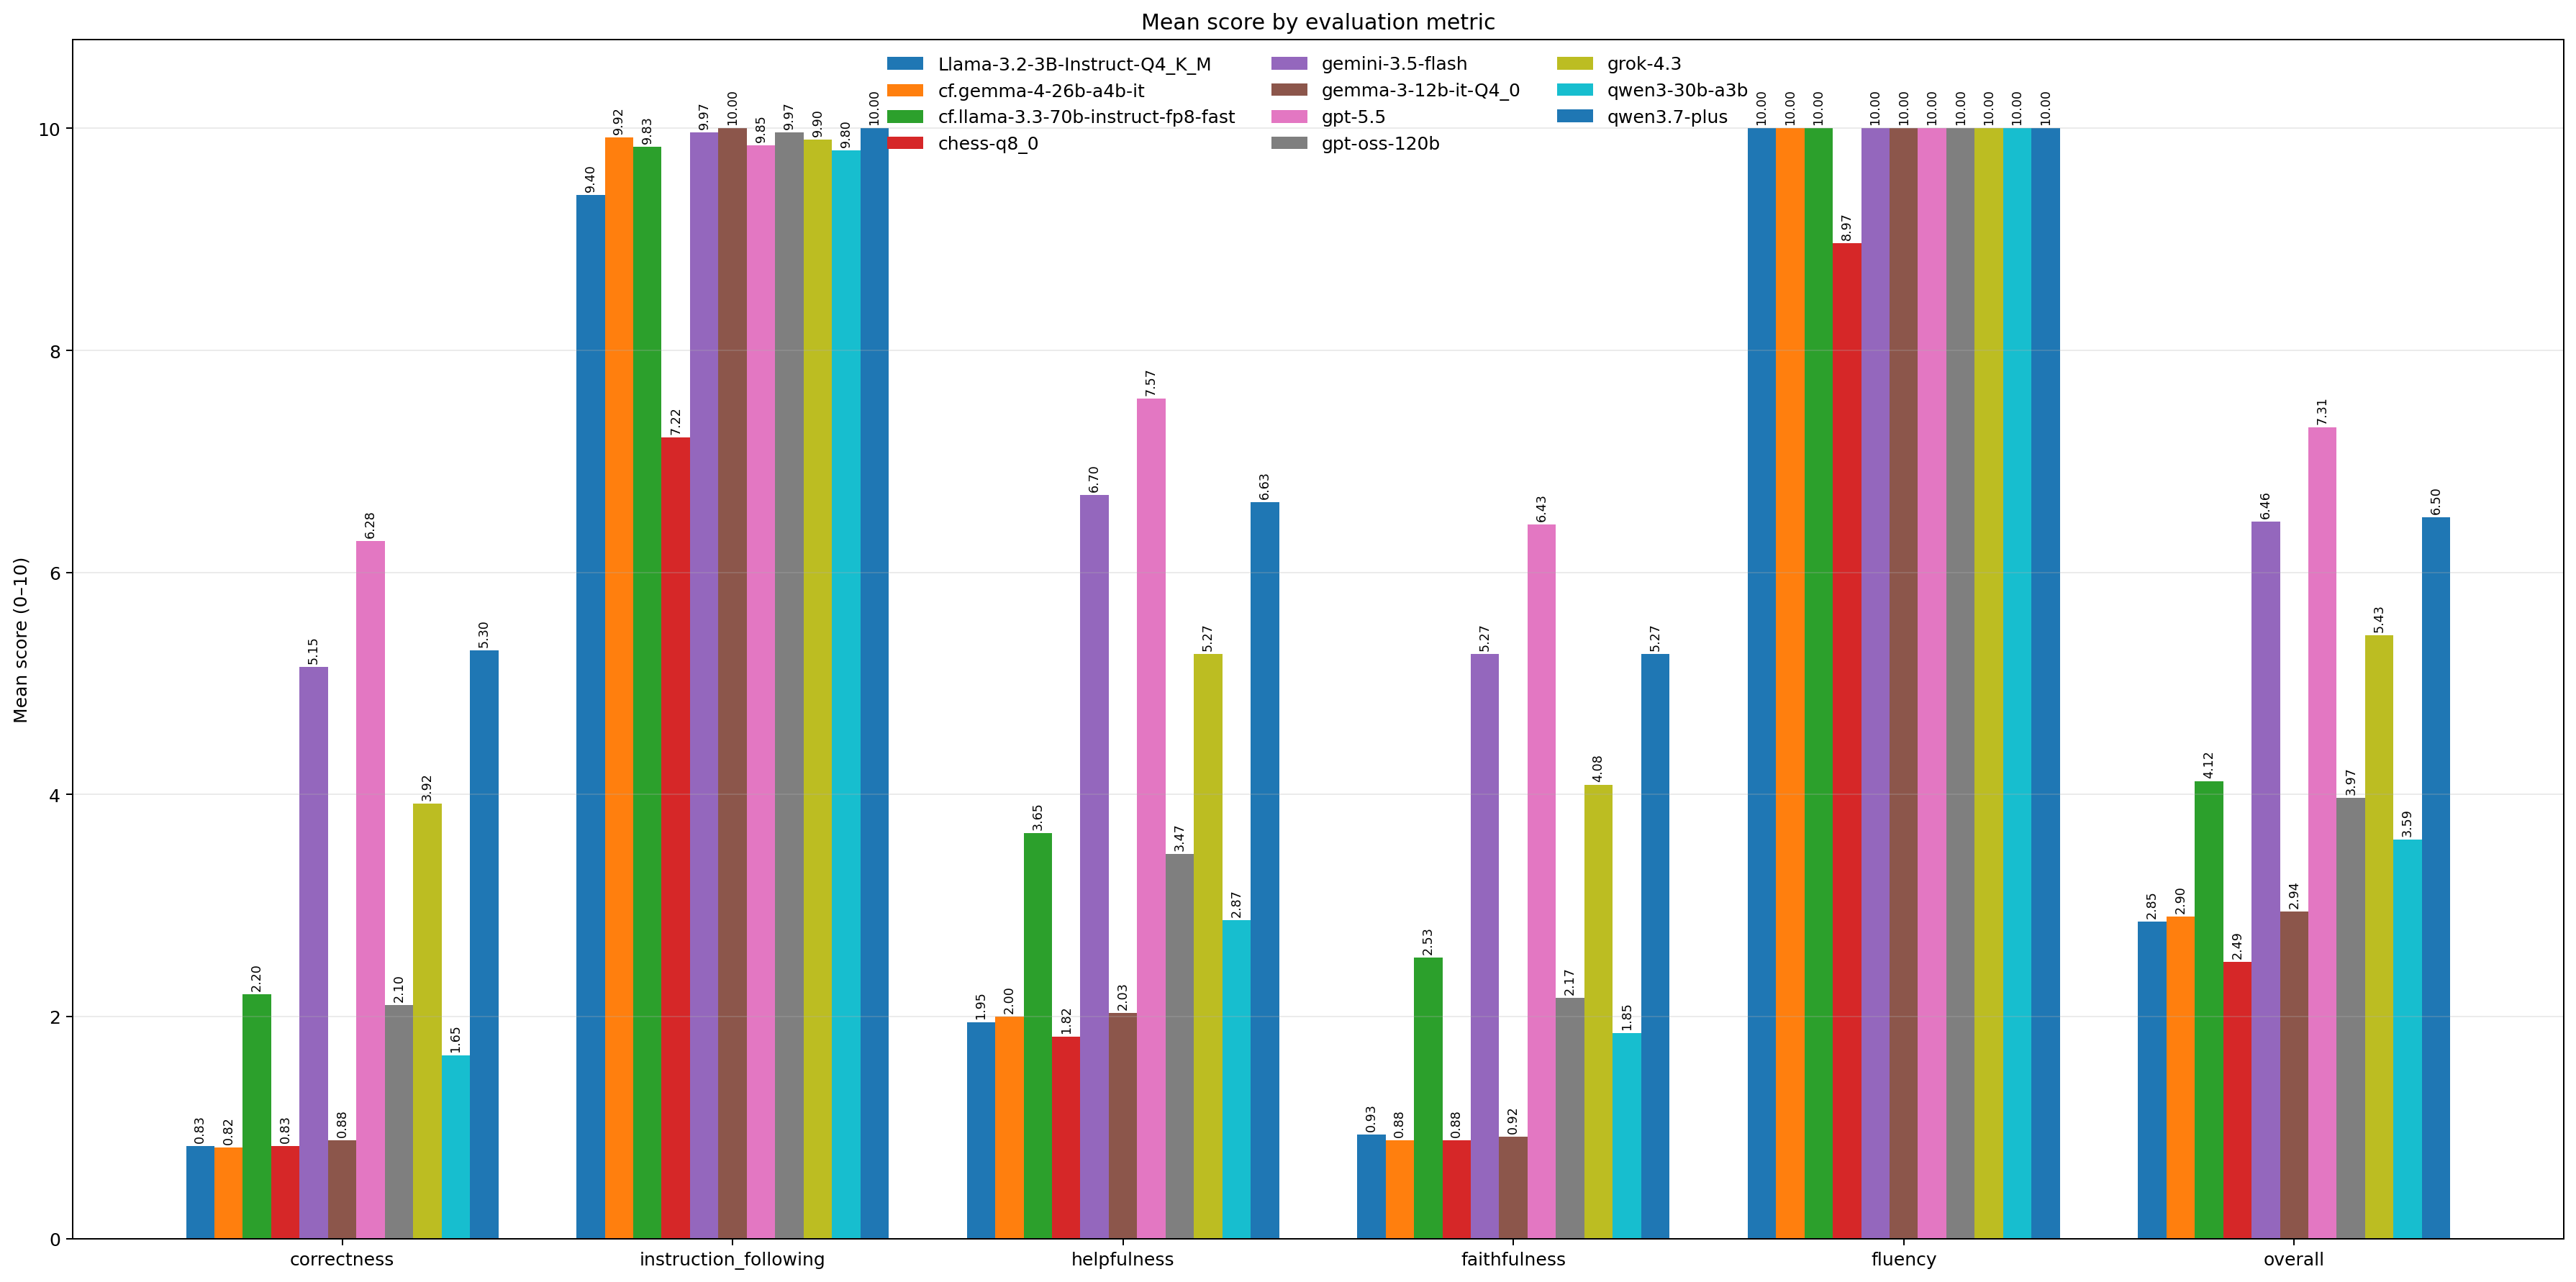
\includegraphics[width=0.85\textwidth]{gemma4_judge_plots/01_metric_means.png}
    \caption{میانگین امتیازات معیارها برای مدل‌های پاسخ‌دهنده، ارزیابی‌شده تنها توسط داور Gemma-4-12B.}
    \label{fig:metric-means}
\end{figure}

\begin{figure}[htbp]
    \centering
    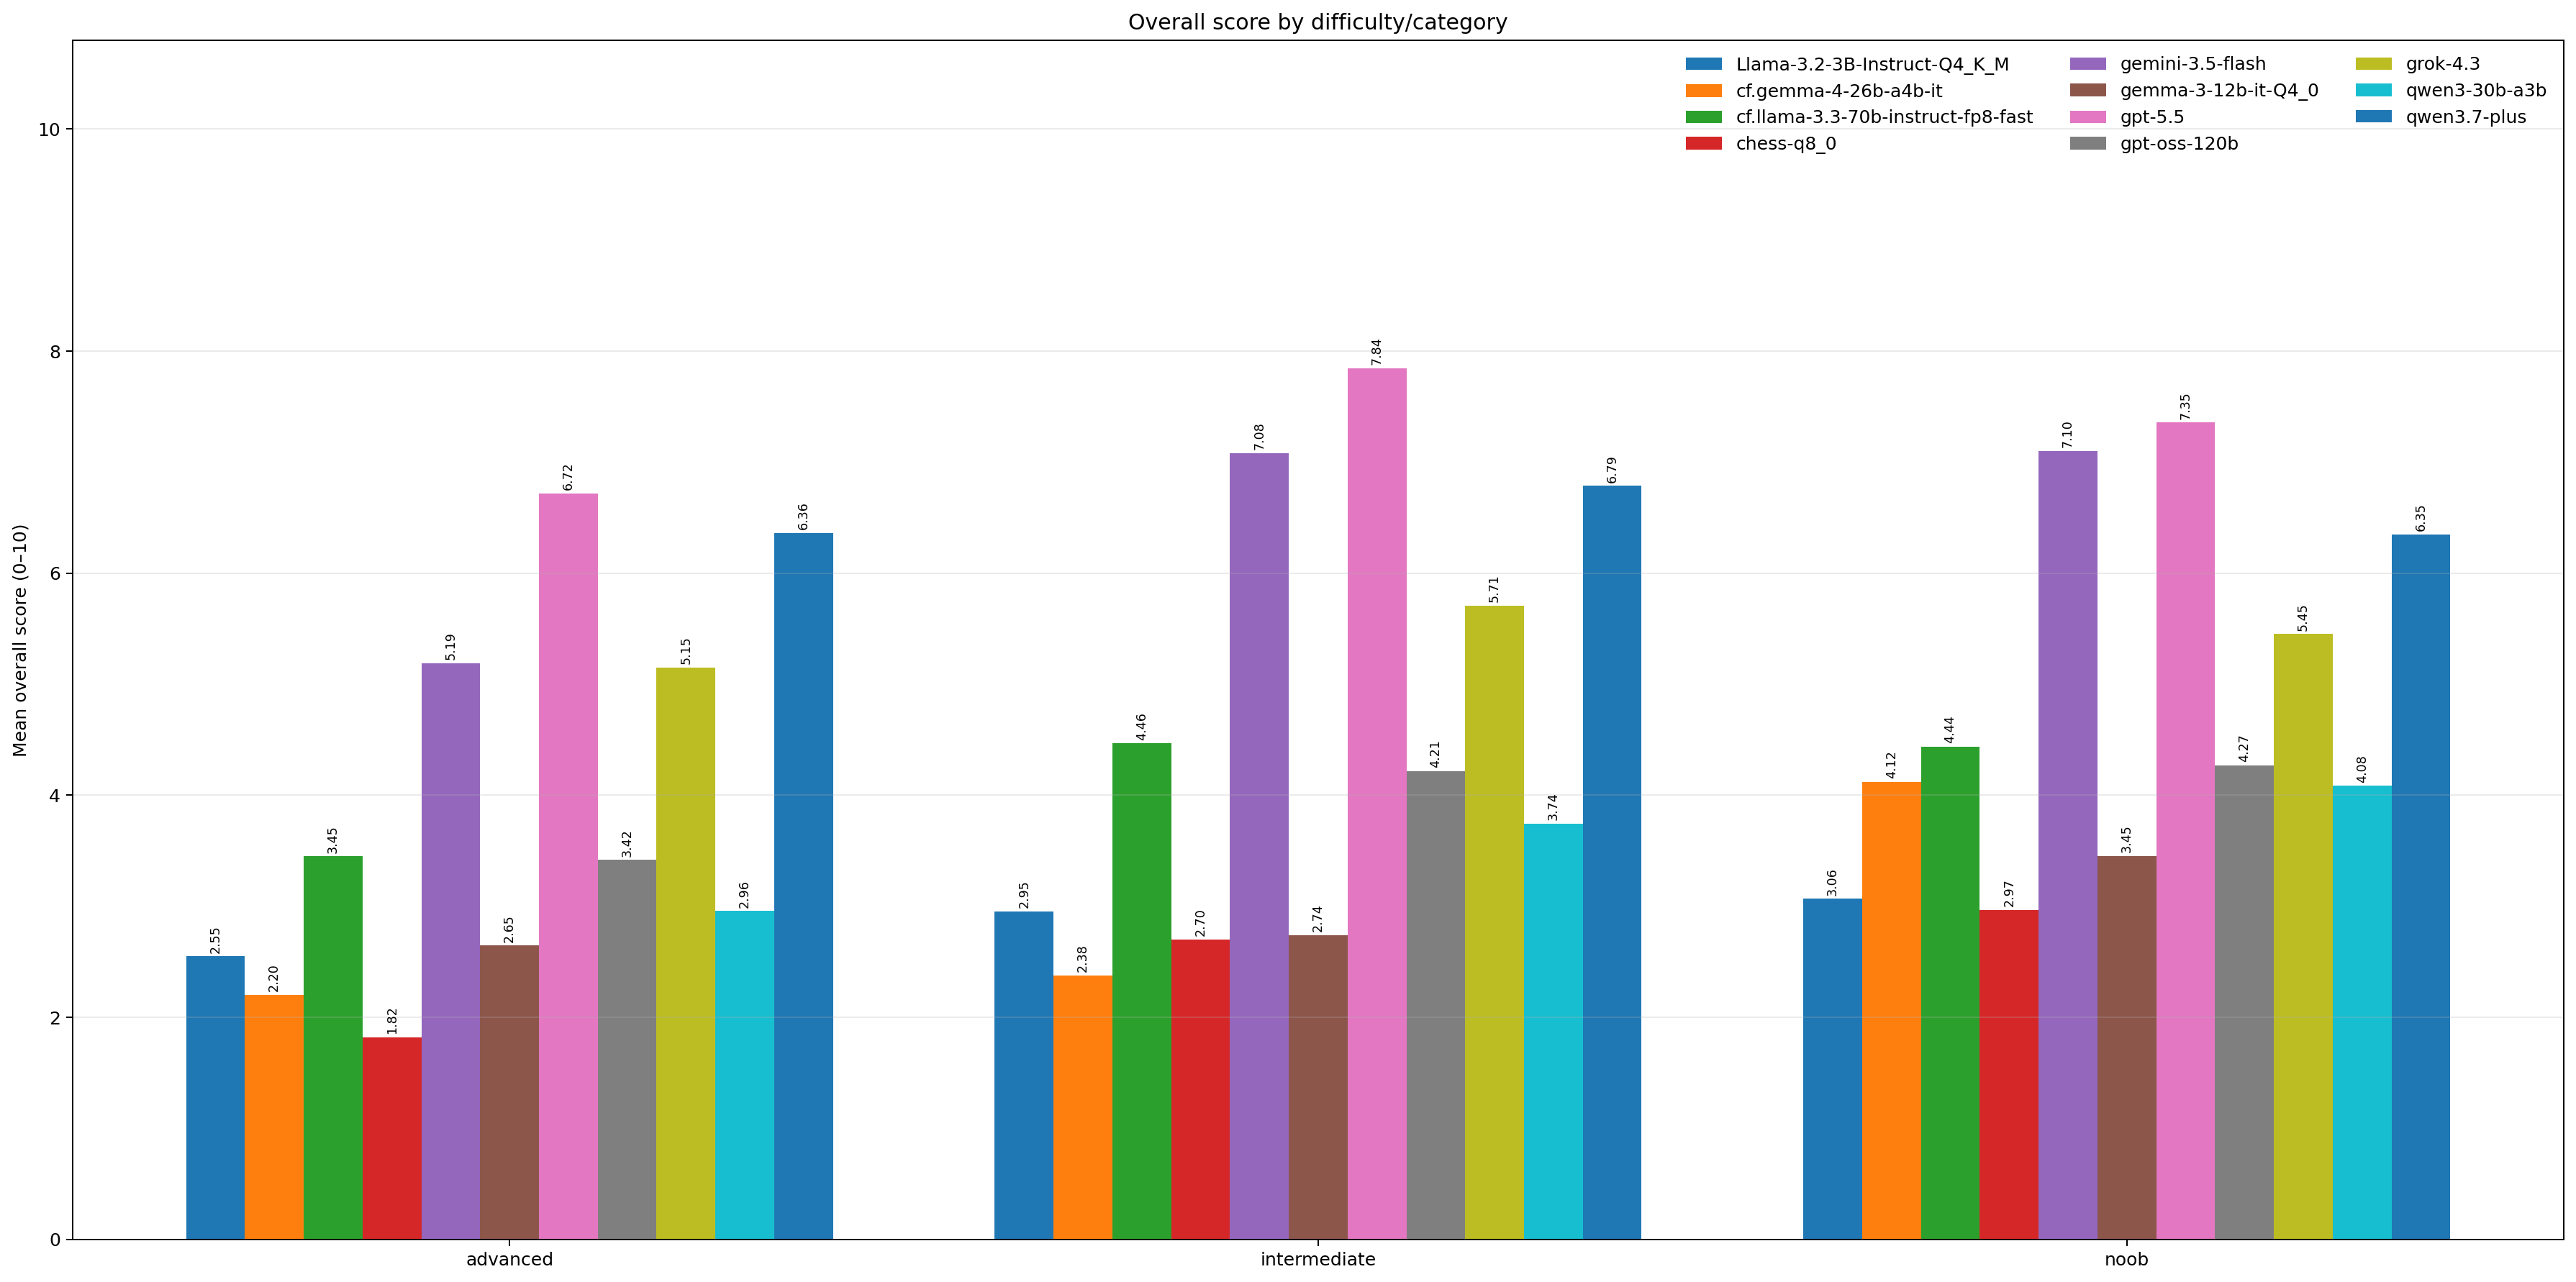
\includegraphics[width=0.75\textwidth]{gemma4_judge_plots/02_category_comparison.png}
    \caption{میانگین امتیاز کلی وزن‌دار بر اساس دشواری معیار. هر مدل ۲۰ موقعیت در هر گروه دارد.}
    \label{fig:category-results}
\end{figure}

\section{بحث و نتیجه‌گیری}
نگهبان خطا یک خط لوله سبک و کامل برای ترکیب شواهد موتور کلاسیک با تولید زبان را نشان می‌دهد، اما ارزیابی کمی یک محدودیت کیفیت واضح را شناسایی می‌کند. مدل تنظیم‌شده از طراحی استقرار محلی پیروی می‌کند، اما شواهد ارائه‌شده را به طور قابل اعتماد به توضیحات شطرنجی هم‌راستا با مرجع ترجمه نمی‌کند.
\textbf{نتیجه‌گیری اصلی} روش‌شناختی است: پایه‌سازی موتور ضروری است، اما پرامپت فعلی و تنظیم دقیق بر روی کتاب‌های جفت‌نشده تضمین نمی‌کند که یک مدل کوچک از آن شواهد به درستی استفاده کند. برای استقرار به عنوان یک سیستم آموزشی قابل اعتماد، آموزش مبتنی بر موقعیت، معیارهای بزرگتر، مطالعات ablation و کالیبراسیون انسانی ضروری است.

% --------------------------------------------------
% References
% --------------------------------------------------
\begin{thebibliography}{99}
\bibitem{stockfish}
Stockfish Developers, \textit{Stockfish Chess Engine}, https://stockfishchess.org.

\bibitem{dettmers2023qlora}
Dettmers, T., et al. (2023). \textit{QLoRA: Efficient Finetuning of Quantized LLMs}. arXiv preprint arXiv:2305.14314.

\bibitem{lichesselite}
Lichess, \textit{Lichess Elite Database}, https://database.lichess.org.

\bibitem{pythonchess}
Niklas Fiekas, \textit{python-chess: A chess library for Python}, https://python-chess.readthedocs.io.

\bibitem{gemma4}
Google DeepMind, \textit{Gemma 4 Technical Report}, 2024.

\bibitem{jhamtani2018chess}
Jhamtani, H., et al. (2018). \textit{Learning to Generate Move-by-Move Commentary for Chess Games from Large-Scale Forums}. ACL.

\bibitem{kim2025ccc}
Kim, et al. (2025). \textit{Concept-guided Chess Commentary}.
\end{thebibliography}

\end{document}